\subsection{Теорема о непрерывном D-оптимальном плане}
	Модель наблюдений:
	\begin{gather} \label{model:start}
		y_i = \theta_0 + \theta_1 x_{i1} + \theta_2 x_{i2} + \varepsilon(x^{(i)}), i = \overline{1, n}, n \ge 3 \\
		E\{ \varepsilon(x^{(i)}) \} = 0, E\{ \varepsilon^{(i)}\ \varepsilon^{(j)} \} = 0, i \ne j \\
		D\{ \varepsilon(x^{(i)}) \} = d(x_{i1}, x_{i2}) > 0, \\
		d(x_1, x_2) \ge \frac{\sigma^2}{3}(1 + x_1^2 + x_2^2) \label{model:end}
	\end{gather}
		$$ -1 \le x_{ij} \le 1, j = \overline{1, 2}, i = \overline{1, n}$$
	Для дисперсии наблюдений $d(x_1, x_2)$ предполагается, что:
	\begin{equation}\label{model:dispersion}
		d(x_1, x_2) \ge \frac{\sigma^2}{3}(1 + x_1^2 + x_2^2), \sigma > 0.
	\end{equation}

	Причем \eqref{model:dispersion} обращается в равенство в вершинах спектра плана:
	\begin{equation}\label{plan-points}
		\begin{gathered}
		x^{(1)}=(1, 1); \\
		x^{(2)}=(-1, 1); \\
		x^{(3)}=(-1, -1); \\
		x^{(4)}=(1, -1)
		\end{gathered}
	\end{equation}
	Введём обозначния: $d(x^{(1)}) = d_1, d(x^{(2)}) = d_2, d(x^{(3)}) = d_3, d(x^{(4)}) = d_4$
		
	\begin{theorem}\label{main-theorem}[о непрерывном D-оптимальном плане в точках спектрах плана]
		Для модели наблюдений \eqref{model:start}-\eqref{model:end} с не коррелированными ошибками наблюдений, имеющими средние значения ноль и дисперсии $d(x_1, x_2)$, следующие планы являются непрерывными $D$-оптимальными. План
		\begin{equation} \label{main-theorem:plan-1}
			\varepsilon_1^{0} = \left \{ 
				\underset{\frac 1 3} {x^{(1)}},
				\underset{\frac 1 3} {x^{(2)}},
				\underset{\frac 1 3} {x^{(3)}}
			\right \}
		\end{equation}
		с дисперисиями наблюдений
		\begin{equation}
			d(x_1, x_2) \ge \frac 1 4 (d_1 + d_3 + 2 d_1 x_1 - 2 d_3 x_2 - 2d_2 x_1 x_2 + (d_1 + d_2)x_1^2 + (d_2 + d_3)x_2^2).
		\end{equation}
		
		План
		\begin{equation}
			\varepsilon_2^{0} = \left \{ 
				\underset{\frac 1 3} {x^{(2)}},
				\underset{\frac 1 3} {x^{(3)}},
				\underset{\frac 1 3} {x^{(4)}}
			\right \}
		\end{equation}
		с дисперисиями наблюдений
		\begin{equation}
			d(x_1, x_2) \ge \frac 1 4 (d_2 + d_4 + 2 d_4 x_1 + 2 d_2 x_2 + 2 d_3 x_1 x_2 + (d_3 + d_4)x_1^2 + (d_2 + d_3)x_2^2).
		\end{equation}
		
		План
		\begin{equation}
			\varepsilon_3^{0} = \left \{ 
				\underset{\frac 1 3} {x^{(1)}},
				\underset{\frac 1 3} {x^{(3)}},
				\underset{\frac 1 3} {x^{(4)}}
			\right \}
		\end{equation}
		с дисперисиями наблюдений
		\begin{equation}
			d(x_1, x_2) \ge \frac 1 4 (d_1 + d_3 - 2 d_3 x_1 + 2 d_1 x_2 - 2 d_4 x_1 x_2 + (d_3 + d_4)x_1^2 + (d_1 + d_4)x_2^2).
		\end{equation}
		
		План
		\begin{equation}
			\varepsilon_4^{0} = \left \{ 
				\underset{\frac 1 3} {x^{(1)}},
				\underset{\frac 1 3} {x^{(2)}},
				\underset{\frac 1 3} {x^{(4)}}
			\right \}
		\end{equation}
		с дисперисиями наблюдений
		\begin{equation}
			d(x_1, x_2) \ge \frac 1 4 (d_2 + d_4 - 2 d_2 x_1 - 2 d_4 x_2 + 2 d_1 x_1 x_2 + (d_1 + d_2)x_1^2 + (d_1 + d_4)x_2^2).
		\end{equation}
		(\ref{main-theorem}) описывает непрерывный D-оптимальный план для модели (6)-(8) в точках $x^{(3)}, x^{(4)}, x^{(1)}$.\\
	\end{theorem}
	\textbf{Доказательство}.
	Опишем вначале процесс построения непрерывного D-оптимального плана $\varepsilon_3^0$.
	Для оптимального плана  $\varepsilon_1^{0}$, по теореме эквивалентности Кифера - Вольфовица [5], выполняется неравенство:
	\begin{equation}\label{main-theorem:ineq}
		\frac 1 {d(x_1, x_2)}
		(1, x_1, x_2)
		M^{-1}(\varepsilon_1^0)
		\begin{pmatrix}1 \\ x_1 \\ x_2 \end{pmatrix} \le 3,
		|x_1| \le 1, |x_2| \le 1,
	\end{equation}
	где $d(x_1, x_2)$ - непрерывная функция, определяющая дисперсию ошибки наблюдения в точке (x1, x2), $M(\varepsilon_1^{0})$ - информационная матрица плана экспериментов. В точках спектра плана $\varepsilon_1^{0}$ неравенство \eqref{main-theorem:ineq}, как необходимое условие, обращается в равенство. Исходя из этих условий, построим класс функций $d(x_1, x_2)$, определяющих поведение дисперсии ошибок наблюдений  для плана $\varepsilon_1^{0}$. Информационная матрица плана $\varepsilon_1^{0}$ равна:
	\begin{gather*}
		M(\varepsilon_1^0) = \frac 1 3 \left(
			\frac 1 d_1 \begin{pmatrix} 1 \\ 1 \\ 1 \end{pmatrix} (1, 1, 1) + 
			\frac 1 d_2 \begin{pmatrix} 1 \\ -1 \\ 1 \end{pmatrix} (1, -1, 1) + 
			\frac 1 d_3 \begin{pmatrix} 1 \\ -1 \\ -1 \end{pmatrix} (1, -1, -1)
		\right) \\ =
		\frac 1 3 
		\begin{pmatrix}
			a & b & c \\
			b & a & e \\
			c & e & a
		\end{pmatrix},
	\end{gather*}
	где
	\begin{equation}\label{main-theorem:defs} \begin{split}
		a=d_1^{-1}+d_2^{-1}+d_3^{-1},\\
		b=d_1^{-1}-d_2^{-1}-d_3^{-1},\\
		c=d_1^{-1}+d_2^{-1}-d_3^{-1},\\
		d=d_1^{-1}-d_2^{-1}+d_3^{-1}.
	\end{split}\end{equation}
	Тогда обратная к матрице $M(\varepsilon_1^0)$ имеет вид:
	\begin{equation} \label{main-theorem:inv-matrix}
		M^{-1}(\varepsilon_1^0) = \frac 3 {a^3 + 2 b c e - a(b^2 + c^2 + e^2)}
		\begin{pmatrix}
			a^2 - e^2,& ce - ab, & be - ac\\
			ce - ab,& a^2-c^2,& bc-ae\\
			be - ac,& bc - ae,& a^2 - b^2			
		\end{pmatrix} 
	\end{equation}.
	Разрешая неравенство \eqref{main-theorem:ineq} относительно $d(x_1, x_2)$ с учетом \eqref{main-theorem:inv-matrix} получим класс функций $d(x_1, x_2)$, определяющих изменение
	дисперсии наблюдений в плане $\varepsilon_1^0$:
	\begin{equation} \label{main-theorem:d-f-ineq}
		d(x_1, x_2) \ge f(x_1, x_2)
	\end{equation}
	где
	\begin{multline}
		f(x_1, x_2) =
			\frac {1}{a^3 + 2bce - a(b^2+c^2+e^2)} \times \\
		\times [{a^2 - e^2 +2(ce - ab)x_1 + 2(be-ac)x_2 + 2(bc - ae)x_1 x_2 + (a^2 - c^2)x_1^2 + (a^2 - b^2)x_2^2}].		
	\end{multline}
	Если теперь в функции $f(x_1, x_2)$ вернуться к исходным обозначениям \eqref{main-theorem:defs}, то неравенство \eqref{main-theorem:d-f-ineq} обратится в неравенство \eqref{main-theorem:plan-1}. Необходимое условие оптимальности плана также выполняется, так как в точках спектра плана $x^{(1)}, x^{(2)}, x^{(3)}$  неравенство \eqref{main-theorem:plan-1} обращается в равенство.
	
	Справедливость теоремы для планов $\varepsilon_2^0, \varepsilon_3^0,\varepsilon_4^0$ доказывается аналогично, однако меняются обозначения \eqref{main-theorem:defs}.\\ Для $\varepsilon_2^0$:
		\begin{equation*} \begin{split}
			a=d_2^{-1}+d_3^{-1}+d_4^{-1},\\
			b=-d_2^{-1}-d_3^{-1}+d_4^{-1},\\
			c=d_2^{-1}-d_3^{-1}-d_4^{-1},\\
			d=-d_2^{-1}+d_3^{-1}-d_4^{-1};
		\end{split}\end{equation*}
	для $\varepsilon_3^0$:
		\begin{equation*} \begin{split}
			a=d_1^{-1}+d_3^{-1}+d_4^{-1},\\
			b=d_1^{-1}-d_3^{-1}+d_4^{-1},\\
			c=d_1^{-1}-d_3^{-1}-d_4^{-1},\\
			d=d_1^{-1}+d_3^{-1}-d_4^{-1};
		\end{split}\end{equation*}
	для $\varepsilon_4^0$:
		\begin{equation*} \begin{split}
			a=d_1^{-1}+d_2^{-1}+d_4^{-1},\\
			b=d_1^{-1}-d_2^{-1}+d_4^{-1},\\
			c=d_1^{-1}+d_2^{-1}-d_4^{-1},\\
			d=d_1^{-1}-d_2^{-1}-d_3^{-1};
		\end{split}\end{equation*}
	\textbf{Теорема доказана}.
			
	
\subsection{Пример применения теоремы}
	Рассмотрим план в точках $x^{(3)}, x^{(4)}, x^{(1)}$.\\
	Пусть $d(x_1, x_2)$ такая, что в указанных точках проходит через поверхность $z = 4 + x_1 + x_2$.
	Тогда
	\begin{gather*}
		d_1 = d(x_1^{(1)}, x_2^{(1)}) = 4 + 1 + 1 = 6 \\
		d_2 = d(x_1^{(2)}, x_2^{(2)}) = 4 -1 + 1 = 4 \\
		d_3 = d(x_1^{(3)}, x_2^{(3)}) = 4 -1 - 1 = 2 \\
		d_4 = d(x_1^{(4)}, x_2^{(4)}) = 4 + 1 - 1 = 4
	\end{gather*}
	Используя доказанную теорему, можно получить, что
		$$d(x_1, x_2) \ge 2 - x_1 + 3x_2 -2x_1x_2 +\frac{3}{2}x_1^2 + \frac 5 2 x_2^2.$$
	Канонический вид поверхности (эллиптический параболоид):\\
		$$x^2 (4 - \sqrt{5}) + y^2 (4 + \sqrt 5) = 2z$$
	График поверхности:\\
		\begin{center}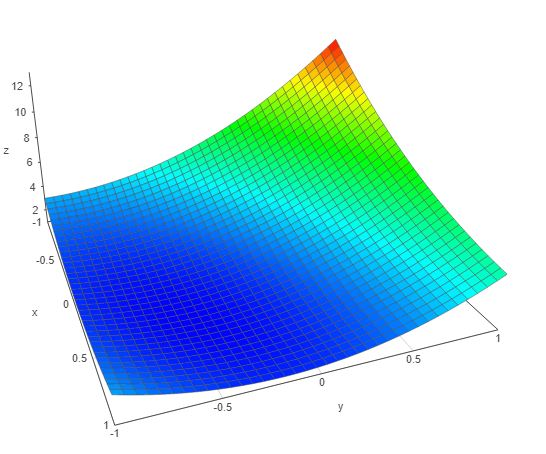
\includegraphics[scale=0.5]{plot134.jpg}\end{center}
		
	Используя аналогичные рассуждения, для остальных планов можно получить:
	\begin{enumerate}
		\item Для плана в точках $x^{(1)}, x^{(2)}, x^{(3)}$:
			$$d(x_1, x_2) \ge 2 + 3x_1 - x_2 -2x_1x_2 +\frac{5}{2}x_1^2 + \frac 3 2 x_2^2.$$
			Канонический вид поверхности:
						$$x^2 (4 - \sqrt{5}) + y^2 (4 + \sqrt 5) = 2z$$
			График поверхности:\\
					\begin{center}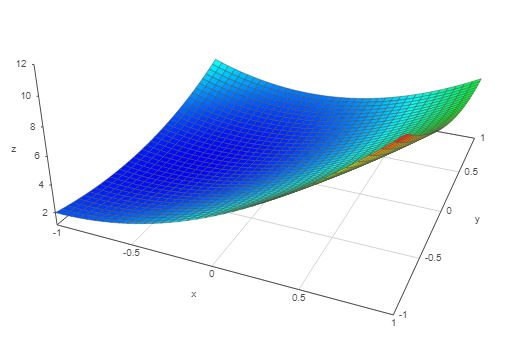
\includegraphics[scale=0.5]{plot123.jpg}\end{center}
			
		\item План в точках $x^{(1)}, x^{(2)}, x^{(4)}$:
			$$d(x_1, x_2) \ge 2 - 2x_1 - 2x_2 +3x_1x_2 +\frac{5}{2}x_1^2 + \frac 5 2 x_2^2$$
				Канонический вид поверхности:
						$$x^2 + 4y^2 = z$$
			График поверхности:\\
					\begin{center}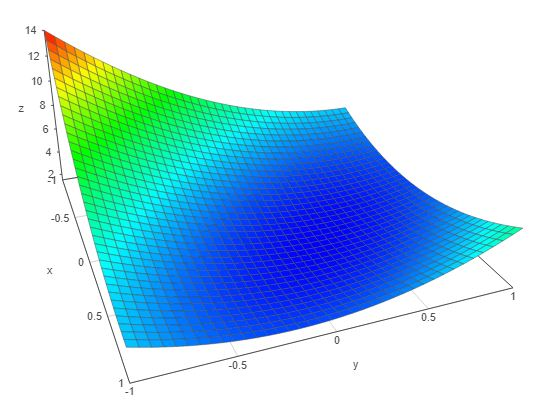
\includegraphics[scale=0.5]{plot124.jpg}\end{center}
		\item План в точках $x^{(2)}, x^{(3)}, x^{4)}$:
			$$d(x_1, x_2) \ge 2 + 2x_1 + 2x_2 +x_1x_2 +\frac{3}{2}x_1^2 + \frac 3 2 x_2^2$$
			Канонический вид поверхности:
						$$x^2 + 2 y^2 = z$$
			График поверхности:\\
					\begin{center}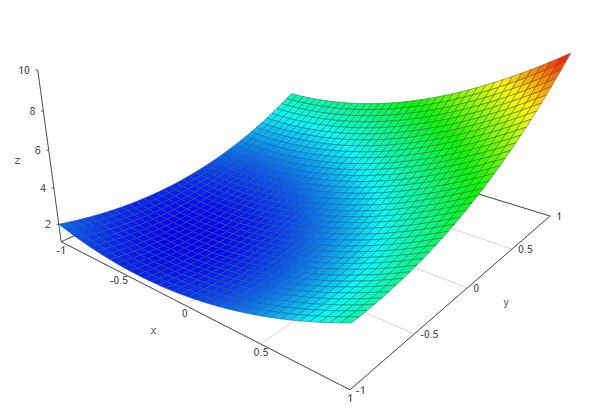
\includegraphics[scale=0.5]{plot234.jpg}\end{center}
	\end{enumerate}
	
\subsection{Программная проверка оптимальности}
	Подтвердим полученные результаты практически. Для этого была написана программа, которая перебирает все возможные планы исходной задачи и находит оптимальный.\\
	Программа написана на языке Python с использованием пакетов numpy, scipy.\\
	Приведем ее исходный код:
	\lstinputlisting[language=Python,tabsize=2]{listings/check_optimal_in_points.py}

	Вывод программы:
	\lstinputlisting[numbers=none]{listings/check_optimal_in_points_output.txt}
	Результат работы программы подтверждает теоретические рассуждения.

	
\subsection {Символьная проверка оптимальности}
	 В предыдыщем параграфе оптимальность построенных планов была показана численно для заданной функции дисперсии. Покажем символьно, что неравенство \eqref{main-theorem:ineq} действительно обращается в равенство в вершинах спектра плана.\\
	Для доказательства этого факта была написана программа в среде Matlab.
	Указанная программа проверяет, что построенные планы в вершинах спектра плана в точности обращаются в значение дисперсии в заданной точке.
	Приведём её листинг:
	\lstinputlisting[language=Matlab,tabsize=2]{listings/symbol_check_optimality.txt}
	
	Результат работы программы:
	\lstinputlisting[numbers=none]{listings/symbol_check_optimality_output.txt}
	
	Видно, что равенства выполняются.
	
\subsection {Точный D-оптимальный план для неравноточной модели наблюдений, сосредоточенный во всех вершинах куба}
	Ранее нам удалось построить точные $D$-оптимальные планы, рассматривая 3 вершины спектра плана. Возникает вопрос: можно ли построить точный $D$-оптимальный план для неравноточной модели наблюдений на всех 4-х вершинах спектра плана? Ответ на данный вопрос дает следующая
	\begin{theorem} \label{theorem-4p}
		Для модели неравноточных наблюдений \eqref{model:start}-\eqref{model:end} с некоррелированными ошибками
		не существует точного $D$-оптимального плана вида:
		\begin{equation}
			\varepsilon^{0} = \left \{
				\underset{\frac 1 4} {x^{(1)}},
				\underset{\frac 1 4} {x^{(2)}},
				\underset{\frac 1 4} {x^{(3)}},
				\underset{\frac 1 4} {x^{(4)}}
			\right \}.
		\end{equation}	 
	\end{theorem}
	\textbf{Доказательство.}
	Для доказательства теоремы необходимо показать, что для указанного плана не будет выполняться критерий оптимальности:
	\begin{equation}\label{theorem-4p:criterion}
		\frac 1 {d(x_1, x_2)}
			(1, x_1, x_2)
			M^{-1}(\varepsilon_1^0)
			\begin{pmatrix}1 \\ x_1 \\ x_2 \end{pmatrix} \le 3,
			|x_1| \le 1, |x_2| \le 1,
	\end{equation}
	Составим информационную матрицу плана $M(\varepsilon^0)$:
	\begin{multline*}
		M(\varepsilon^0) = \\ 
		\frac 1 4 \left(
			\frac 1 d_1 \begin{pmatrix} 1 \\ 1 \\ 1 \end{pmatrix} (1, 1, 1) + 
			\frac 1 d_2 \begin{pmatrix} 1 \\ -1 \\ 1 \end{pmatrix} (1, -1, 1) + 
			\frac 1 d_3 \begin{pmatrix} 1 \\ -1 \\ -1 \end{pmatrix} (1, -1, -1) +
			\frac 1 d_4 \begin{pmatrix} 1 \\ 1 \\ -1 \end{pmatrix} (1, 1, -1)
		\right) \\ =
		\frac 1  4
		\begin{pmatrix}
			a & b & c \\
			b & a & e \\
			c & e & a
		\end{pmatrix},
	\end{multline*}
	где
	\begin{equation}\label{theorem-4p:defs} \begin{split}
		a=d_1^{-1}+d_2^{-1}+d_3^{-1} + d_4^{-1},\\
		b=d_1^{-1}-d_2^{-1}-d_3^{-1} + d_4^{-1},\\
		c=d_1^{-1}+d_2^{-1}-d_3^{-1} - d_4^{-1},\\
		e=d_1^{-1}-d_2^{-1}+d_3^{-1} - d_4^{-1}.
	\end{split}\end{equation}
	С помощью пакета символьной математики \textbf{Sympy} найдём вид обратной матрицы $M^{-1}(\varepsilon^0)$:
	\begin{equation} \label{theorem-4p:inv-matrix}
		M^{-1}(\varepsilon^0) = \frac 4 {a^3 + 2 b c e - a(b^2 + c^2 + e^2)}
		\begin{pmatrix}
			a^2 - e^2,& ce - ab, & be - ac\\
			ce - ab,& a^2-c^2,& bc-ae\\
			be - ac,& bc - ae,& a^2 - b^2			
		\end{pmatrix} 
	\end{equation}.	
	
	Далее перепишем \eqref{theorem-4p:criterion} относительно $d(x_1, x_2)$, подставим туда выражение \eqref{theorem-4p:inv-matrix} и при помощи пакета \textit{Sympy} вернёмся к $d_1, d_2, d_3, d_4$ согласно \eqref{theorem-4p:defs}. Получим:
	\begin{gather*}
		d(x_1, x_2) \ge \frac 1 {3 (d_1 + d_2 + d_3 + d_4)} 
		[ 
			(d_1 d_3 + d_1 d_4 + d_2 d_3 + d_2 d_4) x_1^2 + \\
			(d_1 d_2 + d_1 d_3 + d_2 d_4 + d_3 d_4) x_2^2 + \\
			2 (d_1 d_3 - d_2 d_4) x_1 x_2 +
			2 (d_1 d_4 - d_2 d_3) x_1 + \\
			2 (d_1 d_2 - d_3 d_4) x_2 +
			(d_1 d_2 + d_1 d_4 + d_2 d_3 + d_3 d_4)
		].
	\end{gather*}
	Учтем, что \eqref{theorem-4p:criterion} должно обращаться в равенство в вершинах куба, получим систему уравнений относительно $d_1, d_2, d_3, d_4$:
	\begin{gather*}
		d(1, 1) = \frac 4 3 \frac {d_1 (d_2 + d_3 + d_4)} {d_1 + d_2 + d_3 + d_4} = d_1 \\
		d(-1, 1) = \frac 4 3 \frac {d_2(d_1 + d_3 + d_4)} {d_1 + d_2 + d_3 + d_4} = d_2 \\
		d(-1, -1) = \frac 4 3 \frac {d_3 (d_1 + d_2 + d_4)} {d_1 + d_2 + d_3 + d_4} = d_3 \\
		d(1, -1) = \frac 4 3 \frac {d_4 (d_1 + d_2 + d_3)} {d_1 + d_2 + d_3 + d_4} = d_4.
	\end{gather*}
	Данная система имеет единственное решение $d_1 = d_2 = d_3 = d_ 4 = 1$, при этом решении наблюдения являются равноточнымы, что противоречит предположению о неравноточности наблюдений.
	\textbf{Теорема доказана}.
	
\subsection{Точный D-оптимальный план для модели с линейным изменением}
	
	Рассмотрим следующую модель наблюдений:
	\begin{equation} \label{linear-model:start}
		y_i = \theta_0 + \theta_1 x_{i1} + \theta_2 x_{i2} + \varepsilon(x^{(i)}), |x_{i j}| \le 1, i = \overline{1, n}, j = \overline{1, 2}
	\end{equation}
	\begin{equation} \begin{split}
		E\{\varepsilon(x^{(i)}) \varepsilon(x^{(j)}) \} = 0, i \ne j \\
		E\{\varepsilon(x^{(i)}) = 0
	\end{split}\end{equation}
	\begin{equation}\label{linear-model:end}
		D\{ \varepsilon( x^{(i)} ) \} = a_0 + a_1 x_{i1} + a_2 x_{i2},
		a_0 > 0, |a_1| + |a_2| < a_0
	\end{equation}
	Справедлива следующая теорема.
	\begin{theorem}
		Для модели наблюдений \eqref{linear-model:start}-\eqref{linear-model:end} существует точный $D$-оптимальный план, точки спектра которого лежат в вершинах единичного квадрата.
	\end{theorem}
	Доказательство данной теоремы может быть найдено в \cite{kirlitsa2017}.
	Точный D-оптимальный план при заданном $n$ будет иметь следующий вид:
	\begin{equation}
		\varepsilon^{0} = \left \{ 
			\underset{n_1} {x^{(1)}},
			\underset{n_2} {x^{(2)}},
			\underset{n_3} {x^{(3)}},
			\underset{n_4} {x^{(4)}},
		\right \}
	\end{equation}
	где $n_i$ - число наблюдений, которое нужно провести в точке $x^{(i)}$.\\
	Однако числа $n_1, n_2, n_3, n_4$ не известны. Составим программу, которая для заданной функции дисперсии будет находить оптимальное размещение наблюдений в вершинах спектра плана.
	Для этого воспользуемся тем фактом, что оптимальный план максимизирует определитель информационной матрицы Фишера $M(\varepsilon)$:
	\begin{multline*} 
		M(\varepsilon) = \sum_{i = 1}^{4} \frac{n_i} {d_i} 
		\begin{pmatrix}1 \\ x_{i1} \\ x_{i2} \end{pmatrix}
		(1, x_{i1}, x_{i2}) = \\
		= \frac {n_1} {d_1} \begin{pmatrix}1 \\ 1 \\ 1\end{pmatrix} (1, 1, 1) + 
		\frac {n_2} {d_2} \begin{pmatrix}1 \\ -1 \\ 1\end{pmatrix} (1, -1, 1) + \\
		+ \frac {n_3} {d_3} \begin{pmatrix}1 \\ -1 \\ -1\end{pmatrix} (1, -1, -1) +
		\frac {n_4)} {d_4} \begin{pmatrix} 1 \\ 1 \\ -1\end{pmatrix} (1, 1, -1) = \\
		= \begin{pmatrix}
			\lambda_1 + \lambda_2 + \lambda_3 + \lambda_4 &&
			\lambda_1 - \lambda_2 - \lambda_3 + \lambda_4 &&
			\lambda_1 + \lambda_2 - \lambda_3 - \lambda_4
			\\
			\lambda_1 - \lambda_2 - \lambda_3 + \lambda_4 &&
			\lambda_1 + \lambda_2 + \lambda_3 + \lambda_4 &&
			\lambda_1 - \lambda_2 + \lambda_3 - \lambda_4
			\\
			\lambda_1 + \lambda_2 - \lambda_3 - \lambda_4 &&
			\lambda_1 - \lambda_2 + \lambda_3 - \lambda_4 &&
			\lambda_1 + \lambda_2 + \lambda_3 + \lambda_4
		\end{pmatrix} = \\
		= \begin{pmatrix}
			a && b && c \\
			b && a && e \\
			c && e && a
		\end{pmatrix},
	 \end{multline*}
	 где
	\begin{gather*}
		\lambda_i = \frac {n_i} {d_i}, \\
		a, b, c, e - \text{ соответствующие элемементы матрицы }.
	\end{gather*}
	 Формулы для вычисления определителя подобной матрицы были получены нами ранее.
	 
	 Тогда для нахождения оптимального плана необходимо перебрать различные наборы $n_1, n_2, n_3, n_4$ и посмотреть, какие из них максимизируют определитель информационной матрицы. Именно это и делает следующая программа на языке Python:
	 
	\lstinputlisting[language=Python]{listings/check_ns.py}
	 
	 Вывод программы:
	 \lstinputlisting[numbers=none]{listings/check_ns_output.txt}


	Для каждой поверхности $d(x_1, x_2)$ программа выводит массив оптимальных размещений наблюдений \textit{best placements}, каждый элемент которого есть $[n1, n2, n3, n4]$ -  количесто наблюдений в точках $x^{(1)}, x^{(2)}, x^{(3)}, x^{(4)}$ соответственно.\\
	Проанализируем полученные результаты.\\
	$n = 5$.\\
	В первом случае рассматривается поверхность $d(x_1, x_2) \ge 40 + 0*x_1 + 0*x_2$, то есть равноточные наблюдения. В таких условиях существует 4 оптимальных плана, при которых в 3-х вершинах спектра по 1-му наблюдению и 2 наблюдения в 4-ой точке. \\
	Далее рассматривается поверхность $d(x_1, x_2) \ge 40 - 1*x_1 + 0*x_2$. Видим, что при незначительном наклоне поверхности оптимальный план не изменяется. \\
	Однако в случае $d(x_1, x_2) \ge 40 - 8*x_1 + 0*x_2$ существует уже только 2 оптимальных плана: 2 наблюдения размещаются в "менее поднятых" вершинах.\\
	В критическом случае $d(x_1, x_2) \ge 40 - 39.5*x_1 + 0*x_2$ существует всего 1 оптимальный план.
	
\subsection{Модель с тремя независимыми переменными}
	Выше была рассмотрена модель линейной регрессии \eqref{model:start}-\eqref{model:end} с 3-мя параметрами и 2-мя независимыми переменными.
	Обобщим данную модель, вводя третью независимую переменную $x_0$:
	\begin{gather} \label{model-3x:start}
		y_i = \theta_0 x_{i0} + \theta_1 x_{i1} + \theta_2 x_{i2} + \varepsilon(x^{(i)}), i = \overline{1, n}, n \ge 3 \\
		E\{ \varepsilon(x^{(i)}) \} = 0, E\{ \varepsilon^{(i)}\ \varepsilon^{(j)} \} = 0, i \ne j \\
		D\{ \varepsilon(x^{(i)}) \} = d(x_{i0}, x_{i1}, x_{i2}) > 0, \\
		d(x_0, x_1, x_2) \ge \frac{\sigma^2}{3}(x_0^2 + x_1^2 + x_2^2) \label{model-3x:end},
		-1 \le x_{ij} \le 1, j = \overline{0, 2}, i = \overline{1, n},
	\end{gather}
	где $n$ - число наблюдений, $x_{ij}$ - независимые переменные, $x^{(i)} = (x_{i0}, x_{i1}, x_{i2})^T$ - вектор наблюдений, $\varepsilon(x^{(i)})$ - случайные некоррелированные ошибки.
	
	Таким образом все наблюдения находятся внутри куба c центром в точке $(0, 0, 0)$ и стороной 2.
	Занумеруем вершины куба:
	\begin{align*}
		x^{(1)} = (1, 1, 1), && x^{(2)} = (1, -1, 1), && x^{(3)} = (1, -1, -1), && x^{(4)} = (1, 1, -1),\\
		x^{(5)} = (-1, 1, 1), && x^{(6)} = (-1, -1, 1), && x^{(7)} = (-1, -1, -1), && x^{(8)} = (-1, 1, -1).
	\end{align*}
	Точки $x^{(1)}-x^{(4)}$ лежат на верхней грани куба и обозначены так же, как в модели \eqref{model:start}-\eqref{model:end}.\\
	Также обозначим значение функции дисперсии в вершинах куба:
	\begin{equation}
		d_i = d(x^{(i)}), i = \overline{1, 8}.
	\end{equation}
	
	В теореме \ref{main-theorem} было показано, что для модели с двумя независимыми переменными \eqref{model:start}-\eqref{model:end} можно построить трёхточеный $D$-оптимальный план.  
	Попробуем построить трёхточечный $D$-оптимальный план для модели тремя независимыми переменными  \eqref{model-3x:start}-\eqref{model-3x:end}.
	\begin{theorem}\label{theorem:model-3x-D-opt}
		Для модели неравноточных наблюдений \eqref{model-3x:start}-\eqref{model-3x:end} следующие трехточечные планы являются непрерывными и $D$-оптимальными.\\
		План 
		\begin{equation} \label{theorem:model-3x-D-opt:plan-1}
			\varepsilon_1^{0} = \left \{ 
				\underset{\frac 1 3} {x^{(1)}},
				\underset{\frac 1 3} {x^{(2)}},
				\underset{\frac 1 3} {x^{(3)}}
			\right \},
		\end{equation},
		если для дисперсии наблюдений выполняется:
		\begin{multline}\label{theorem:model-3x-D-opt:plan-1-d}
			d(x_0, x_1, x_2) \ge \frac{d_{2} x_{1} x_{2}}{2} + x_{0}^{2} \left(\frac{d_{1}}{4} + \frac{d_{3}}{4}\right) + x_{0} \left(\frac{d_{1} x_{1}}{2} - \frac{d_{3} x_{2}}{2}\right) + \\ + x_{1}^{2} \left(\frac{d_{1}}{4} + \frac{d_{2}}{4}\right) + x_{2}^{2} \left(\frac{d_{2}}{4} + \frac{d_{3}}{4}\right).
		\end{multline}
		План 
		\begin{equation} \label{theorem:model-3x-D-opt:plan-2}
			\varepsilon_2^{0} = \left \{ 
				\underset{\frac 1 3} {x^{(1)}},
				\underset{\frac 1 3} {x^{(2)}},
				\underset{\frac 1 3} {x^{(4)}}
			\right \},
		\end{equation},
		если для дисперсии наблюдений выполняется:
		\begin{multline}\label{theorem:model-3x-D-opt:plan-2-d}
			d(x_0, x_1, x_2) \ge \frac{d_{1} x_{1} x_{2}}{2} + x_{0}^{2} \left(\frac{d_{2}}{4} + \frac{d_{4}}{4}\right) + x_{0} \left(- \frac{d_{2} x_{1}}{2} - \frac{d_{4} x_{2}}{2}\right) + \\ + x_{1}^{2} \left(\frac{d_{1}}{4} + \frac{d_{2}}{4}\right) + x_{2}^{2} \left(\frac{d_{1}}{4} + \frac{d_{4}}{4}\right).
		\end{multline}
		План 
		\begin{equation} \label{theorem:model-3x-D-opt:plan-3}
			\varepsilon_3^{0} = \left \{ 
				\underset{\frac 1 3} {x^{(1)}},
				\underset{\frac 1 3} {x^{(3)}},
				\underset{\frac 1 3} {x^{(4)}}
			\right \},
		\end{equation},
		если для дисперсии наблюдений выполняется:
		\begin{multline}\label{theorem:model-3x-D-opt:plan-3-d}
			d(x_0, x_1, x_2) \ge \frac{d_{4} x_{1} x_{2}}{2} + x_{0}^{2} \left(\frac{d_{1}}{4} + \frac{d_{3}}{4}\right) + x_{0} \left(\frac{d_{1} x_{2}}{2} - \frac{d_{3} x_{1}}{2}\right) + \\ + x_{1}^{2} \left(\frac{d_{3}}{4} + \frac{d_{4}}{4}\right) + x_{2}^{2} \left(\frac{d_{1}}{4} + \frac{d_{4}}{4}\right).
		\end{multline}
		План 
		\begin{equation} \label{theorem:model-3x-D-opt:plan-4}
			\varepsilon_4^{0} = \left \{ 
				\underset{\frac 1 3} {x^{(2)}},
				\underset{\frac 1 3} {x^{(3)}},
				\underset{\frac 1 3} {x^{(4)}}
			\right \},
		\end{equation},
		если для дисперсии наблюдений выполняется:
		\begin{multline}\label{theorem:model-3x-D-opt:plan-4-d}
			d(x_0, x_1, x_2) \ge \frac{d_{3} x_{1} x_{2}}{2} + x_{0}^{2} \left(\frac{d_{2}}{4} + \frac{d_{4}}{4}\right) + x_{0} \left(\frac{d_{2} x_{2}}{2} + \frac{d_{4} x_{1}}{2}\right) + \\ + x_{1}^{2} \left(\frac{d_{3}}{4} + \frac{d_{4}}{4}\right) + x_{2}^{2} \left(\frac{d_{2}}{4} + \frac{d_{3}}{4}\right).
		\end{multline}		
	\end{theorem}
	
	\textbf{Доказательство}. Доказательство данной теоремы производится аналогично доказательству теоремы \ref{main-theorem}. Для плана в точках $x^{(i)}, x^{(j)}, x^{(k)}$ запишем критерий эквавалентности Кифера-Вольфовица \eqref{theorem:model-3x-D-opt:KF-ineq}:
	\begin{equation}\label{theorem:model-3x-D-opt:KF-ineq}
		\frac{1}{d(x_0, x_1, x_2)} f'(x) M^{-1}(\varepsilon^0) f(x) \le 3
	\end{equation},
	выразим $d(x_0, x_1, x_2)$ и покажем, что $d(x_0, x_1, x_2)$ равно заданным дисперсиям $d_i, d_j, d_k$ в соответствующих точках.
	
	Произведём доказательство при помощи пакета компьютерной алгебры SymPy, написанном на языке Python.
	\lstinputlisting[language=Python, tabsize=2]{listings/3x_cube.py}
	Вывод программы:
	\lstinputlisting[numbers=none]{listings/3x_cube_output.txt}
	Вывод показывает, что неравенство обращается в равенство в вершинах плана. \textbf{Теорема доказана}.\\
	
	\textbf{Замечание}.
	В теореме \ref{theorem:model-3x-D-opt} были рассмотрены планы, точки которых находятся на верхней грани куба. Куб имеет 6 граней, причём на каждой из них можно построить аналогичные планы. Данный факт следует из того, что точки планов на других гранях эквиваленты точкам одного из планов на верхней грани с точностью до переименования независимых переменных $x_0, x_1, x_2$ и домножения на $-1$. Таким образом доказано существование $24$-ых планов для модели \eqref{model-3x:start}-\eqref{model-3x:end}.	
	
	
	
	